\documentclass[letterpaper, 12pt]{article}
\usepackage[letterpaper, top=2.5cm, bottom=2.5cm, left=3cm, right=3cm]{geometry} %margenes
\usepackage[utf8]{inputenc} %manejo de caracteres especiales
\usepackage[spanish]{babel} %manejo de encabezados de inglés a español
\usepackage{fancyhdr} %formato de los encabezados de página
\usepackage{ragged2e} %alineado real justficado
\usepackage{graphicx} %manejo de imagenes
\usepackage{amsmath} %manejo de notación matemática
\usepackage{mathtools} %manejo de notación matemática
\usepackage{blindtext} %texto de relleno
\usepackage{amssymb} %manejo de simbología matematica
\usepackage{float} % centrado de imagenes

\pagestyle{fancy}
\fancyhf{}
\rfoot{}

\begin{document}
\thispagestyle{fancy}
\lhead{\textbf{Nombre: Abraham Jhared Flores Azcona\\\#: 19211640}}
\rhead{Actividad 16\\Parte teórica de la interpolación}
\subsection*{¿Qué es una interpolación?}
\justify
En términos generales, es la inserción de algo de distinta naturales en otra cosa. Por esta definición podemos inferir que la interpolación matemática
consiste en la misma idea. Específicamente hablando en la disciplina matemática, son métodos para acomodar ciertos datos en una curva. 
\\\newline
Por los fines de brevedad, se describe la interpolación lineal que consiste en aproximar una función con una composición de rectas dado un conjunto de puntos de la misma.
\begin{figure}[H]
        \centering
        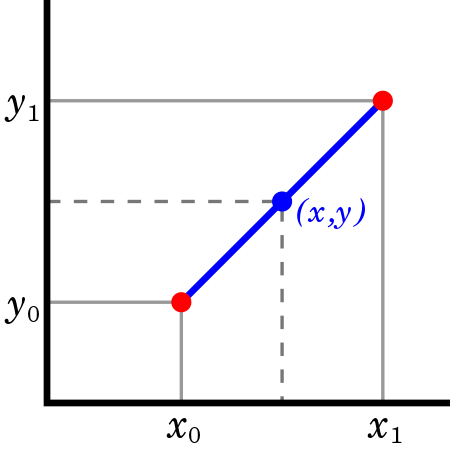
\includegraphics[width=5cm,height=5cm]{450px-LinearInterpolation.png}
\end{figure}
\justify
En la interpolación de Newton (la más simple) se necesitan dos puntos cualquiera (\(x_0, y_0\)) y (\(x_1, f_1\)) y el punto medio (\(x,y\)) se obtiene del planteamiento
de la ecuación de la recta, que se simplifica a las siguientes expresiones:
{\large\[y=y_0+{y_1 - y_0\over x_1-x_0}\,(x-x_0)=y_0\,{x_1-x\over x_1-x_0}+y_1\,{x-x_0\over x_1-x_0}\]}
\justify
Algo relevante a destacar es que su contrario, la extrapolación trata de encontrar datos fuera del rango de los datos conocidos.
\subsection*{¿Qué es una regresión?}
\justify
En términos estadísticos, la regresión es una medida estadística que intenta determinar la fortaleza y el carácter de la relación entre una variable dependiente
y una serie de otras variables, llamadas independientes. 
\\\newline
De manera similar a la repsuesta anterior, se explica de manera breve la regresión lineal simple.
\begin{figure}[H]
    \centering
    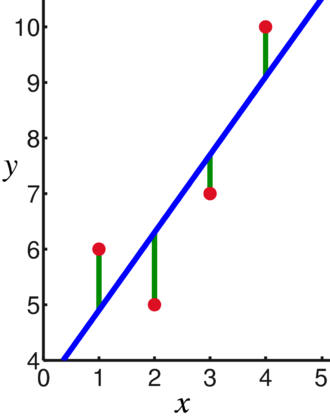
\includegraphics[width=5cm,height=5cm]{330px-Linear_least_squares_example2.png}
\end{figure}
\justify
Para este caso, las observaciones (en color rojo) se asumen que son el resultado de desviaciones aleatorias (en color verde) de una relación (en color azul) entre la variable dependiente (\(y\))
y de una variable independiente (\(x\)). La fórmula general para estas relaciones es:
{\large\[y=X\beta+\epsilon\]}
\justify
Donde \(y\) es el vector de valores observados del regresando, \(X\) es la matriz de vectores columna que representa los valores de entrada, \(\beta\) es el vector de parámetros y \(\epsilon\)
es el vector de valores de ruido.
\subsection*{¿Cuál es la diferencia entre interpolación y regresión?}
\justify
La diferencia fundamental es que \textbf{\emph{la interpolación desea imitar a una función provisto de un conjunto de datos}} mientras que \textbf{\emph{la regresión busca encontrar la relación de un conjunto provisto de datos}}.
\subsection*{¿Qué aplicaciones tiene la interpolación?}
\justify
Como se menciona ante, su principal aplicación es la de aproximar funciones, especialmente aquellas complejas en funciones más simples lo que computacionalmente deriva en ahorros de tiempo en la ejecución de algorítmos computacionales y por ende, la eficiencia de los mismos.
\subsection*{¿Cómo se calcula una interpolación de primer y segundo grado?}
\justify
Se asume que cuando se desea calcular la interpolación de distintos grados, se está hablando de la interpolación polinomial.
\subsubsection*{De primer grado}
\justify
Esta se deriva de la formula de la recta.
{\large\[y=y_0+{y_1 - y_0\over x_1-x_0}\,(x-x_0)=y_0\,{x_1-x\over x_1-x_0}+y_1\,{x-x_0\over x_1-x_0}\]}
\justify
Notese que para este tipo de interpolación se necesitan al menos dos puntos para el cálculo.
\subsubsection*{De segundo grado}
\justify
Acorde al polinomio de Lagrange:
{\large \[f(x)={(x-m)(x-b)\over (a-m)(a-b)}f(a)+{(x-a)(x-b)\over (m-a)(m-b)}f(m)+{(x-a)(x-m)\over (b-a)(b-m)}f(b)\]}
\justify
Donde \(m={a+b\over 2}\).
\\\newline
Notese que para este tipo de interpolación se necesitan al menos dos puntos para el cálculo, el tercero se calcula como la mitad de estos.
\end{document}